\de{ĐỀ THI HỌC KỲ II NĂM HỌC 2022-2023}{THPT Tạ Quang Bữu}

\begin{bt}%[0D7Y3-2]%[Dự án đề kiểm tra HKII NH22-23- Nguyễn Ngọc Dũng]%[Tạ Quang Bửu]
Giải phương trình $\sqrt{8-2x} = 2x-6$.
\loigiai{
Ta có 
\allowdisplaybreaks 
\begin{eqnarray*}
\sqrt{8-2x} = 2x-6 &\Rightarrow& 8-2x = (2x-6)^2 \\
&\Rightarrow& 4x^2-22x+28=0 \\
&\Rightarrow& \hoac{&x=2 \\ &x=\dfrac{7}{2}}
\end{eqnarray*}
Thay lần lượt các giá trị $x=2$ và $x=\dfrac{7}{2}$ vào phương trình đã cho, ta nhận $x=\dfrac{7}{2}$ và loại $x=2$.\\
Vậy $S=\left\{ \dfrac{7}{2} \right\}$.
}
\end{bt}


\begin{bt}%[0D7B2-1]%[Dự án đề kiểm tra HKII NH22-23- Nguyễn Ngọc Dũng]%[Tạ Quang Bửu]
Giải bất phương trình bậc hai sau bằng cách lập bảng xét dấu:
\[3x^2-9x-30 \leq 4x(x-5).\]
\loigiai{
Ta có
$$3x^2-9x-30 \leq 4x(x-5) \Leftrightarrow -x^2+11x-30 \leq 0.$$
Bảng xét dấu
\begin{center}
\begin{tikzpicture}
\tkzTabInit[lgt=4.5,espcl=3]
{$x$ /1, $-x^2+11x-30$ /1}
{$-\infty$,$5$,$6$,$+\infty$}
\tkzTabLine{ ,-,0,+,0,-, }
\end{tikzpicture}
\end{center}
Vậy tập nghiệm của bất phương trình đã cho là $S=(-\infty;5] \cup [6;+\infty)$.
}
\end{bt}

\begin{bt}%[0D8Y1-2]%[Dự án đề kiểm tra HKII NH22-23- Nguyễn Ngọc Dũng]%[Tạ Quang Bửu]
Tại một nhà hàng chuyên phục vụ cơm trưa văn phòng, thực đơn có $6$ món chính, $3$ món phụ và $3$ loại đồ uống. Thực khách có bao nhiêu cách lựa chọn bữa trưa gồm một món chính, một món phụ và một loại đồ uống?
\loigiai{
Số cách lựa chọn bữa trưa gồm một món chính, một món phụ và một loại đồ uống là $6\cdot 3\cdot 3 = 54$ (cách).
}
\end{bt}

\begin{bt}%[0D8Y2-1]%[Dự án đề kiểm tra HKII NH22-23- Nguyễn Ngọc Dũng]%[Tạ Quang Bửu]
Từ các chữ số $0$; $1$; $2$; $3$; $4$; $5$; $6$ có thể lập được bao nhiêu số tự nhiên lẻ có năm chữ số đôi một khác nhau?
\loigiai{
Gọi số cần tìm là $\overline{abcde}$.
\begin{itemize}
\item Chọn $e\in \{1;3;5\}$: có $3$ cách.
\item Chọn $a\neq 0, a\neq e$: có $5$ cách.
\item Chọn $3$ số từ $5$ số còn lại xếp vào vị trí $b$, $c$, $d$: có $\mathrm{A}^3_5=60$ cách.
\end{itemize}	
Vậy có tất cả $3\cdot 5\cdot 60 = 900$ số.
}
\end{bt}

\begin{bt}%[0D8B2-1]%[Dự án đề kiểm tra HKII NH22-23- Nguyễn Ngọc Dũng]%[Tạ Quang Bửu]
Trong một lô $100$ sản phẩm, có $96$ chính phẩm (sản phẩm đạt tiêu chuẩn) và $4$ thứ phẩm (sản phẩm không đạt tiêu chuẩn). Từ $100$ sản phẩm này có bao nhiêu cách lấy ra $3$ sản phẩm mà trong đó có ít nhất một thứ phẩm?
\loigiai{
Chọn $3$ sản phẩm bất kì có $\mathrm{C}^3_{100}=161700$ cách.\\
Chọn $3$ sản phẩm mà không có thứ phẩm nào có $\mathrm{C}^3_{96}=142880$ cách.\\
Suy ra số cách lấy ra $3$ sản phẩm mà trong đó có ít nhất một thứ phẩm là 
$$161700 - 142880 =18820 \text{ (cách).}$$
}
\end{bt}

\begin{bt}%[0H9Y2-2]%[Dự án đề kiểm tra HKII NH22-23- Nguyễn Ngọc Nguyên]%[Tạ Quang Bửu]
Trong mặt phẳng tọa độ $Oxy$, cho tam giác $ABC$ có $A(-2;1)$, $B(3;0)$, $C(5;-6)$. Viết phương trình đường thẳng chứa đường trung tuyến $AM$ ($M$ là trung điểm của $BC$).
\loigiai{
Ta có $M$ là trung điểm của $BC$ nên $M(4;-3)$.\\
Ta cũng có $\overrightarrow{AM}= ( x_M-x_A;y_M-y_A)=(6;-4)$.\\
Đường thẳng $AM$ đi qua $A(-2;1)$ có VTCP $\overrightarrow{u}=(6;-4)$ nên có phương trình là 
\[\heva{&x=-2+6t \\ &y=1-4t} (t\in \mathbb{R})\]
}
\end{bt}

\begin{bt}%[0H9B3-2]%[Dự án đề kiểm tra HKII NH22-23- Nguyễn Ngọc Nguyên]%[Tạ Quang Bửu]
Trong mặt phẳng tọa độ $Oxy$, viết phương trình đường tròn có tâm là điểm $A(-1;2)$ và tiếp xúc với đường thẳng $\Delta \colon 3x-4y-4=0$.
\loigiai{
Gọi $(C)$ là đường tròn cần viết phương trình và $R$ là bán kính của $(C)$.\\
Vì $(C)$ tiếp xúc với $\Delta$ nên
$$R=\mathrm{d} (A, \Delta)= \dfrac{|3 \cdot (-1)-4 \cdot 2 -4|}{\sqrt{3^2+4^2}}=3.$$
Đường tròn $(C)$ tâm $A(-1;2)$ và bán kính $R=3$ có phương trình là $(x+1)^2+(y-2)^2=9$.
}
\end{bt}

\begin{bt}%[0H9Y3-1]%[0H9Y3-3]%[Dự án đề kiểm tra HKII NH22-23- Nguyễn Ngọc Nguyên]%[Tạ Quang Bửu]
Trong mặt phẳng tọa độ $Oxy$, cho đường tròn $(C) \colon x^2+y^2-2x+6y-15=0$.
\begin{enumerate}
\item Tìm tọa độ tâm $I$ và tính bán kính của đường tròn $(C)$.
\item Viết phương trình tiếp tuyến $\Delta$ của đường tròn $(C)$ tại $A(4;1)$.
\end{enumerate}
\loigiai{
\begin{enumerate}
\item Tâm $I(1;-3)$ và bán kính $R=\sqrt{1^2+(-3)^2-(-15)}=5$.
\item Ta có $\overrightarrow{IA}=(3;4)$.\\
Tiếp tuyến $\Delta$ đi qua $A(4;1)$ nhận $\overrightarrow{IA}=(3;4)$ làm VTPT nên có phương trình là
$$3(x-4)+4(y-1)=0 \Leftrightarrow 3x+4y-16=0.$$
\end{enumerate}
}
\end{bt}

\begin{bt}%[0H9Y4-2]%[Dự án đề kiểm tra HKII NH22-23- Nguyễn Ngọc Nguyên]%[Tạ Quang Bửu]
Trong mặt phẳng tọa độ $Oxy$, viết phương trình chính tắc của elip $(E)$ biết tiêu cự bằng $18$ và độ dài trục lớn bằng $24$.
\loigiai{
Giả sử $(E)\colon \dfrac{x^2}{a^2}+\dfrac{y^2}{b^2} = 1$ là phương trình elip cần tìm.\\
Vì $(E)$ có tiêu cự bằng $18$ nên $2c=18$ suy ra $c=9$.\\
Vì $(E)$ có độ dài trục lớn bằng $24$ nên $24=2a$ suy ra $a=12$.\\
Ta cũng có $b=\sqrt{a^2-c^2}=3\sqrt{7}$.\\
Vậy $(E) \colon \dfrac{x^2}{144}+\dfrac{y^2}{63}=1$.
}
\end{bt}